\documentclass{article}

\usepackage{graphicx}
\begin{document}

\title{CS4102 Practical 2: 3D Rendering}
\author{160010069}
\date{23rd April, 2021}

\begin{titlepage}
    \maketitle
    \tableofcontents
\end{titlepage}

\section{Introduction}
For this practical we were required to implement a 3D 
face rendering application by interpolating between 3 
faces and rendering the new face. My implementation uses 
Lambert reflection, flat shading, orthographic projection 
and the painter's algorithm.  

\section{Design and Implementation}
The basic design of the project is based around the 
structure of the given data. Every face 
is made up of triangles, every triangle 
has three points, and every point has a colour. 
The project loads in the average face and the three 
reference faces and then combines that data 
based on the weights given by the user. 

\subsection{Loading the Faces}
The FaceParser and AverageFace classes handle the loading 
of the face data. They basically hold the data in 
the format given in the \verb+.csv+ files,
an array of coordinate offsets for each point in the 
mesh. 

\subsection{Rendering the Faces}
After the reference faces are combined with the 
average face the triangles in the mesh are sorted 
so that the furthest back triangles are drawn first 
a la painter's algorithm. The colour of a triangle 
is found from the average of the colour of its three points 
which is then used in the Lambert shading process. Because we are 
using orthographic projection and the viewing direction is 
perfectly along the z-axis the drawing just takes the 
x and y coordinates of the triangles. The faces 
have to be shrunk and moved before being drawn 
so I implemented some simple translating and 
scaling functions. 

\subsection{Lambert Reflectance}
I calculate the Lambert reflection based on the method given in 
class. The normal to the triangle is calculated 
and then the dot product of the normal and the incident 
light is multiplied by the light intensity  and 
the diffuse coefficient. I took the incident light 
vector to be [0,0,1] (in line with the z-axis), 
the light intensity to be 1 and the diffuse coefficient to be 
1 for all colours.

\subsection{Flat Shading}
The flat shading for this is quite simple. Each triangle 
has only one colour which is found by getting the average colour of 
its three points, and then applying the Lambert reflection to 
that colour. 

\subsection{Weighting the Faces}
The weight calculation based on the triangle 
took a little bit of time to get right 
but I'm happy with my solution. When the 
user clicks on the triangle, three new 
triangles are created, one with each point being replaced 
by the point the user clicked. The area of each of these triangles 
is calculated. Since the sum of these areas has to be 
equal to the area of the original triangle, the weights 
for each face can be found by dividing the area 
of each new triangle by the whole area. This feels
quite neat and it means the weights always sum to 1. 

\section{Evaluation}
My submission meets the requirements for the basic 
specification. I don't have any tests 
as such for this practical, I mainly tested it by hand to make 
sure everything worked as expected. The important thing 
is that it renders faces which is enough to convince me that the 
parts that make up the application work correctly. 

\section{Conclusion}
I'm happy with my solution to this practical. 
I enjoyed working on this and felt it reinforced some of the 
computer graphics concepts we went over in class. 
Unfortunately I didn't have the time to implement any extensions 
which is a shame because there were a lot of interesting ways to 
take this. With more time I would have liked to add the ability to 
rotate the face and move the light source, and/or implement extra shading 
or reflection models. 

\section{Building and Running the Project}
I don't include the face data in my submission 
so my application takes the location of that data 
as a command line argument. 
My application can be run as a standalone \verb+.jar+
file using \verb+Render.jar+.
To run it:
\begin{verbatim}
java -jar Render.jar PATH_TO_DATA_DIR
\end{verbatim}

To use the application, just click somewhere in the 
green triangle in the bottom left to set the 
weights for each face. The closer to a 
corner, the more that face is weighted. 

I also included the Processing \verb-.jar- file 
if you do want to build it from scratch. This 
can be done with:
\begin{verbatim}
javac -cp .:core.jar Render.jar
java -cp .:core.jar Render.jar PATH_TO_DATA_DIR
\end{verbatim}
I added some command line arguments to see the application working 
with various options. The face can be drawn only as a mesh, 
or without using any reflection, or with Lambert reflection. 

To use these arguments:
\begin{verbatim}
java -jar Render.jar DATA_DIR --reflectance ARG
\end{verbatim}
where ARG is one of:
\begin{verbatim}
mesh | none | lambert
\end{verbatim}
mesh draws only the mesh, none draws only the 
average colour, and lambert uses lambert reflection. 

\section{Images}

\begin{figure}[htb]
    \centering
    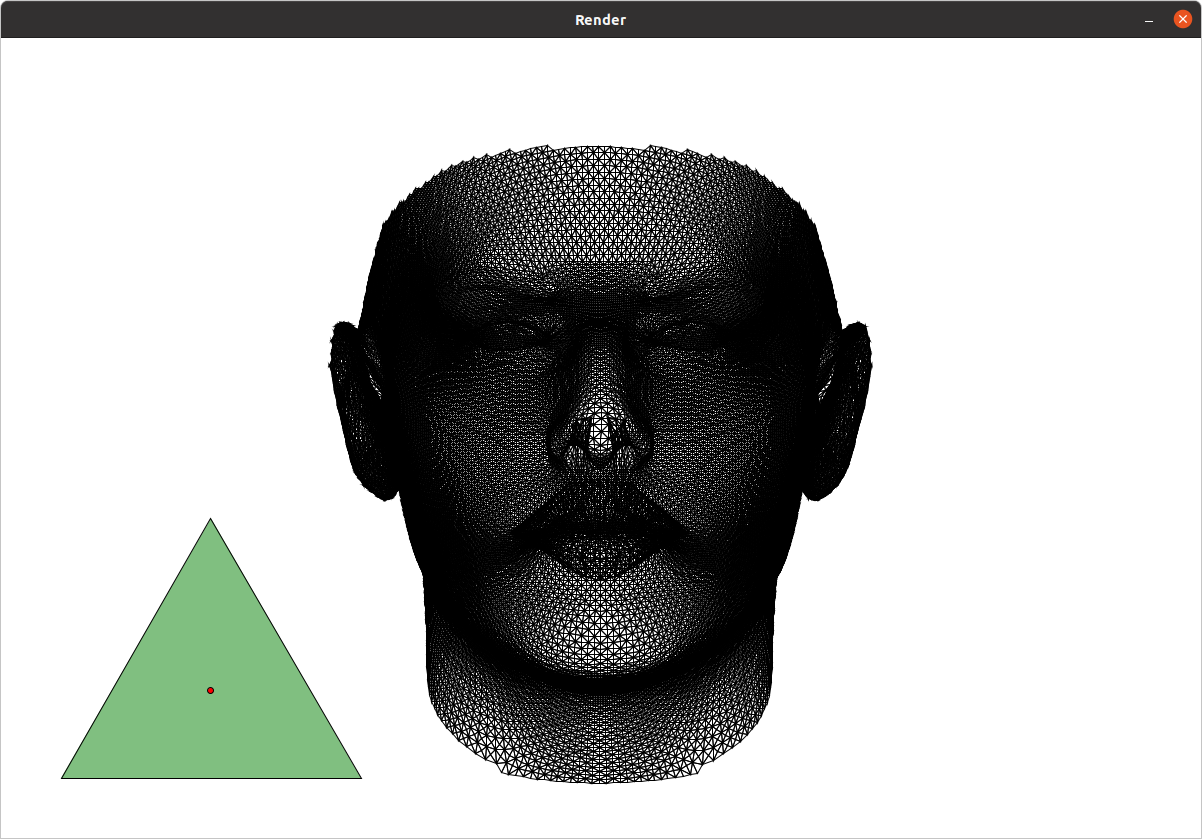
\includegraphics[width=0.6\textwidth]{./images/mesh.png}    
    \caption{The interpolated faces drawn as a mesh.}
    \label{fig:mesh}
\end{figure}
\begin{figure}[htb]
    \centering
    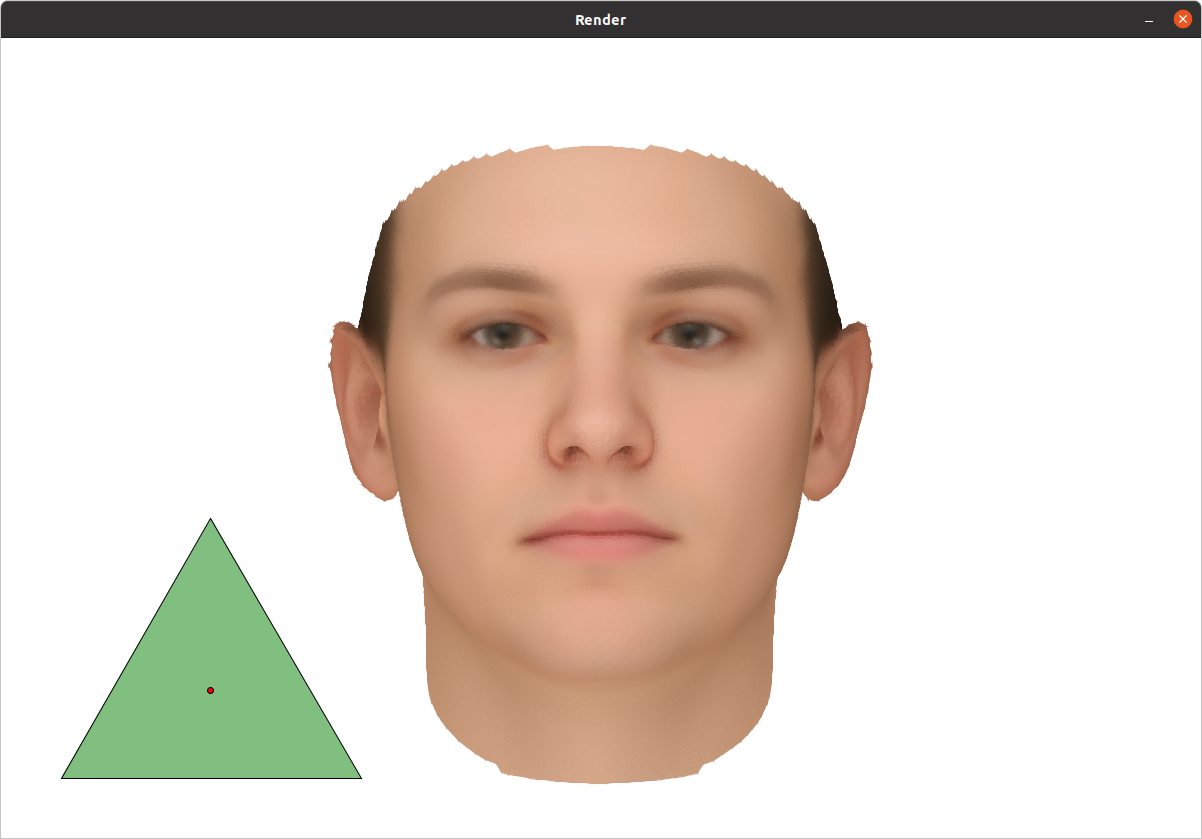
\includegraphics[width=0.6\textwidth]{./images/none.png}
    \caption{The interpolated faces drawn with no reflection.}
    \label{fig:label}
\end{figure}
\begin{figure}[htb]
    \centering
    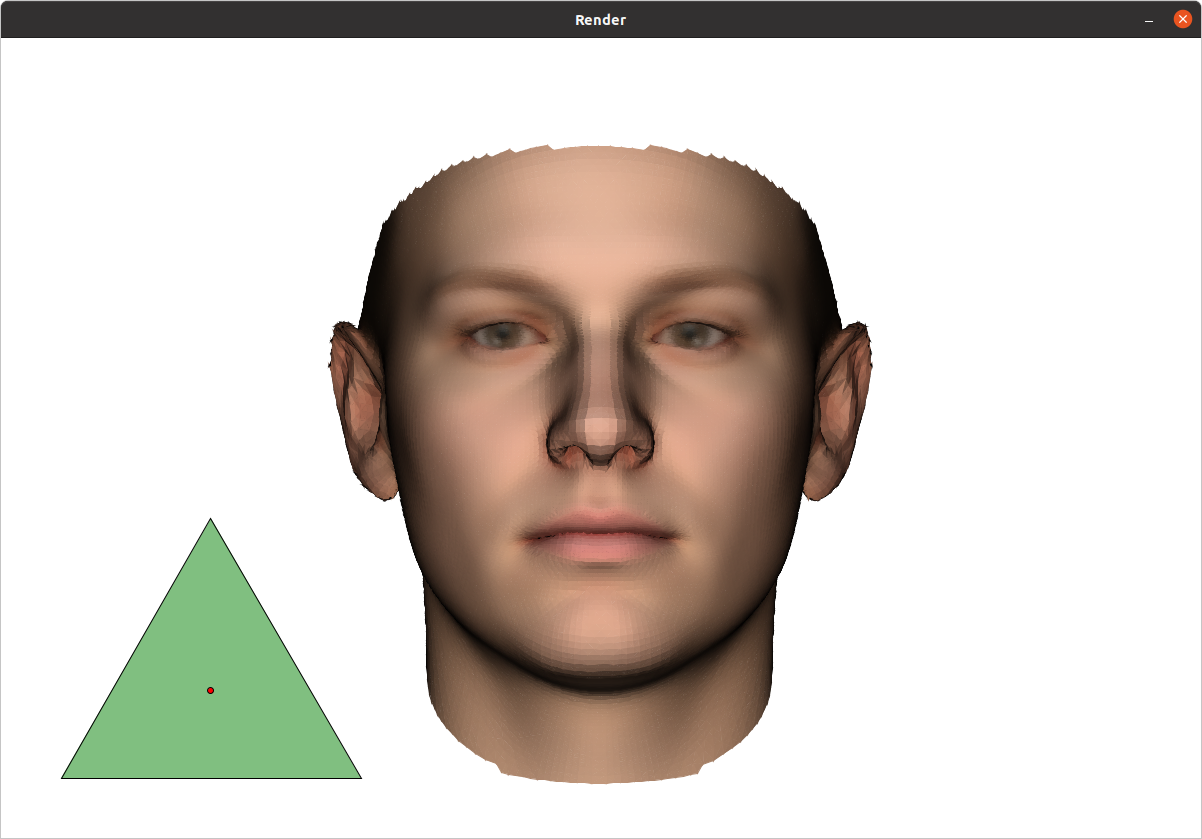
\includegraphics[width=0.6\textwidth]{./images/lambert.png}
    \caption{The interpolated faces drawn with Lambert reflection.}
    \label{fig:label}
\end{figure}
\begin{figure}[htb]
    \centering
    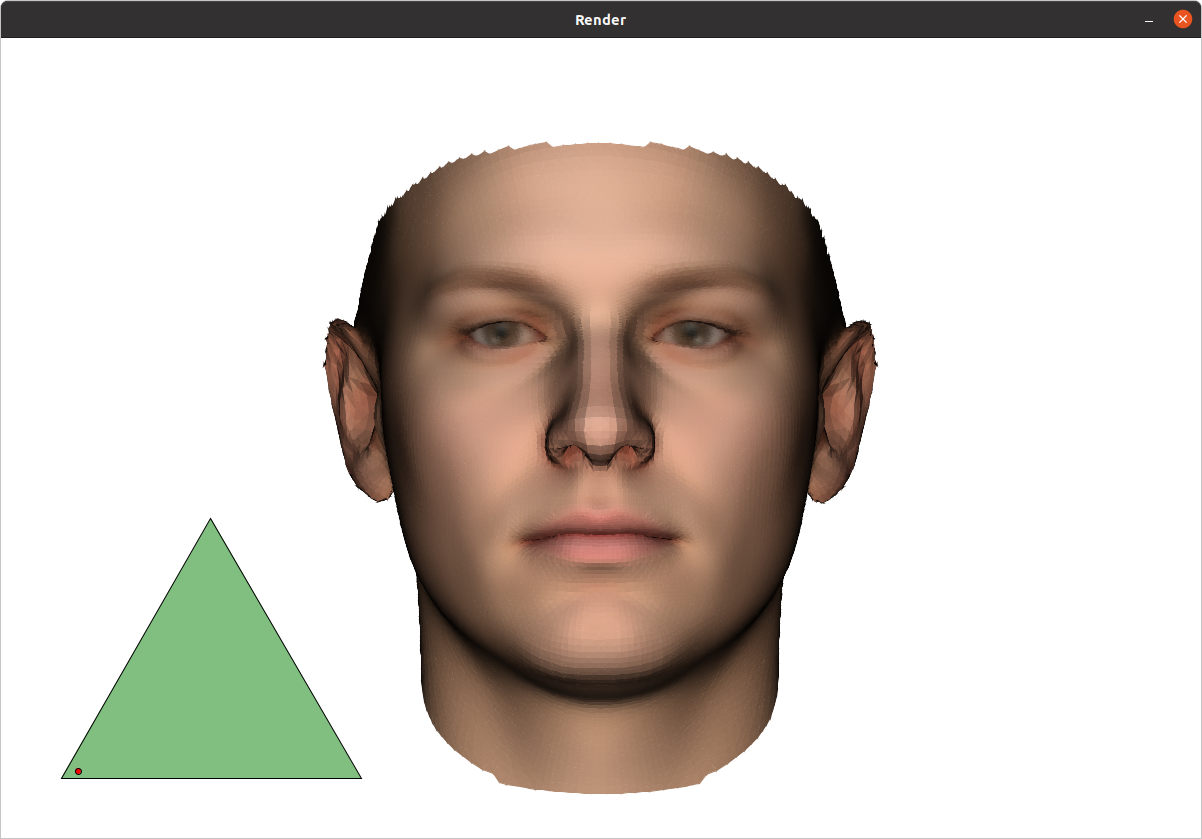
\includegraphics[width=0.6\textwidth]{./images/moved.png}
    \caption{The interpolation point has been moved 
    to change how much each face is weighted. }
    \label{fig:label}
\end{figure}
\end{document}